\chapter{Annexe}

\begin{figure}[h!]
  \center
  \setlength\fboxsep{5pt}
  \setlength\fboxrule{0.5pt}
  \fbox{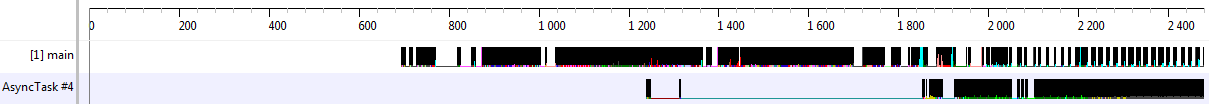
\includegraphics[width=0.9\textwidth]{resources/profiling/method_profiling/Bordeaux1_events.png}}
  \caption{Method profiling montrant le temps nécessaire à parser les événements de Bordeaux 1}
  \label{fig:method_prof1}
\end{figure}

\begin{figure}[h!]
  \center
  \setlength\fboxsep{5pt}
  \setlength\fboxrule{0.5pt}
  \fbox{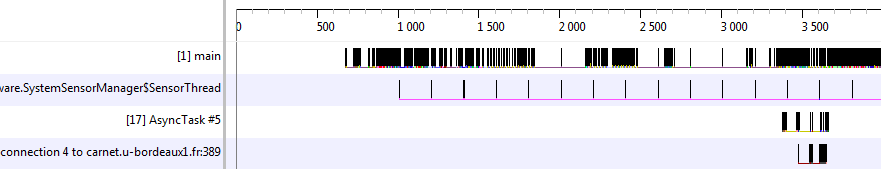
\includegraphics[width=0.9\textwidth]{resources/profiling/method_profiling/Bordeaux1_directory.png}}
  \caption{Method profiling montrant le temps nécessaire pour récupérer les résultats d'une requête auprès du serveur LDAP de Bordeaux 1}
  \label{fig:method_prof2}
\end{figure}

\begin{figure}[h!]
  \center
  \setlength\fboxsep{5pt}
  \setlength\fboxrule{0.5pt}
  \fbox{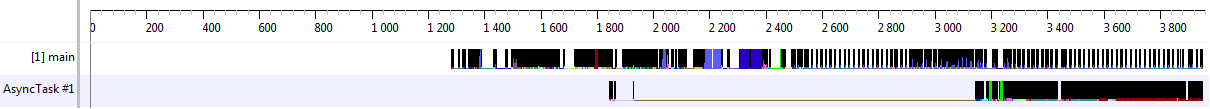
\includegraphics[width=0.9\textwidth]{resources/profiling/method_profiling/Labri_events.png}}
  \caption{Method profiling montrant le temps nécessaire à parser les événements du LaBRI}
  \label{fig:method_prof3}
\end{figure}

\begin{figure}[h!]
  \center
  \setlength\fboxsep{5pt}
  \setlength\fboxrule{0.5pt}
  \fbox{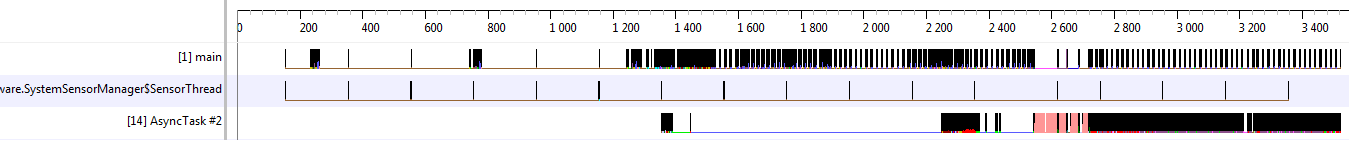
\includegraphics[width=0.9\textwidth]{resources/profiling/method_profiling/Labri_directory.png}}
  \caption{Method profiling montrant le temps nécessaire à parser les contacts du LaBRI}
  \label{fig:method_prof4}
\end{figure}